\chapter{Project Structure} % <<< -------------------------------------------- %
\label{ch:devguide:project_structure}
% ---------------------------------------------------------------------------- %

repo structure: TLDs and what is contained in them.

``Where do I have to go if I want to do X?''

%>>>
\chapter{FPGA/SoC Toolchain} % <<< ----------------------------------------------- %
\label{ch:devguide:fpga_toolchain}
% ---------------------------------------------------------------------------- %

Because the FPGA/SoC requires a lot of different utilities and environments it is advisable to have a fixed development environment as hardware tooling oft breaks at the slightest change.
For this reason we provide a build box which contains a Ubuntu Linux. To set up the build box Vagrant and ansible are required.
The first one pulls the base linux box from a global repository at HashiCorp\footnote{The corporation behind Vagrant}. ansible is then used to provision the box to make it contain all the necessary tooling. Once that is set up, the user has to perform a graphical install of the Vivado Toolchain.

To set up the build box, perform the steps explained in Section~\ref{sec:devguide:sec:devguide:fpga_toolchain:buildbox}

\section{Setting up the buildbox}
\label{sec:devguide:fpga_toolchain:buildbox}

\subsection*{Prerequisites}

Install

\begin{itemize}
    \item Vagrant
    \item ansible
    \item VirtualBox
\end{itemize}

If you are on a Linux or OSX and use a package manager to install VirtualBox it is necessary to also install the Guest Additions packages. They are required in later stages during the setup of the box.
It is also advisible to perform a

\begin{listing}
    \begin{minted}[autogobble]{bash}
        sudo vboxreload
    \end{minted}
\end{listing}

Otherwise a reboot of the host system might be necessary.
After all the tools on the host have been installed, we move to the root of the project repository. For all the further steps we assume that we operate from the root.

To do an initial setup of the box, do

\begin{listing}
    \begin{minted}[autogobble]{bash}
        cd env
        vagrant up
    \end{minted}
\end{listing}

This will boot the box and provision it using ansible. This step requires a stable internet connection. If anything fails during the initial setup (red messages in the shell), you can run and retry the provisioning with

\begin{listing}
    \begin{minted}[autogobble]{bash}
        vagrant provision
    \end{minted}
\end{listing}

Once the provisioning has finished, the build box should be rebootet because some changes (for example the installed desktop environment) require a reboot. Do this by running

\begin{listing}
    \begin{minted}[autogobble]{bash}
        vagrant halt
        vagrant up
    \end{minted}
\end{listing}

If you want to make changes to the default box setup, have a look at \textit{/env/roles/common/tasks/main.yml} and the official ansible\cite{TODO:} documentation.

The fully configured build box should contain two shared folders \textit{/vagrant/} which points to the \textit{/env/} directory on the host and \textit{/repo/} which point to \textit{/} on the host.

\textbf{IMPORTANT:} The password of the default vagrant user is \textbf{vagrant} and can use \textit{sudo}

Now it is time to set up Vivado which is explained in Section~\ref{sec:devguide:fpga_toolchain:vivado}.

\section{Setting up Vivado}
\label{sec:devguide:fpga_toolchain:vivado}

For this Section we assume that we execute all commands on the VirtualBox (guest for the rest of this manual).

Enter

\begin{listing}
    \begin{minted}[autogobble]{bash}
    /repo/Xilinx/Downloads/Xilinx_Vivado_SDK_2016.2_0605_1_Lin64.bin
    \end{minted}
\end{listing}

into a shell to start the Vivado install.
Figure~\ref{} through to Figure~\ref{} guide through the install.

\begin{figure}
    \centering
    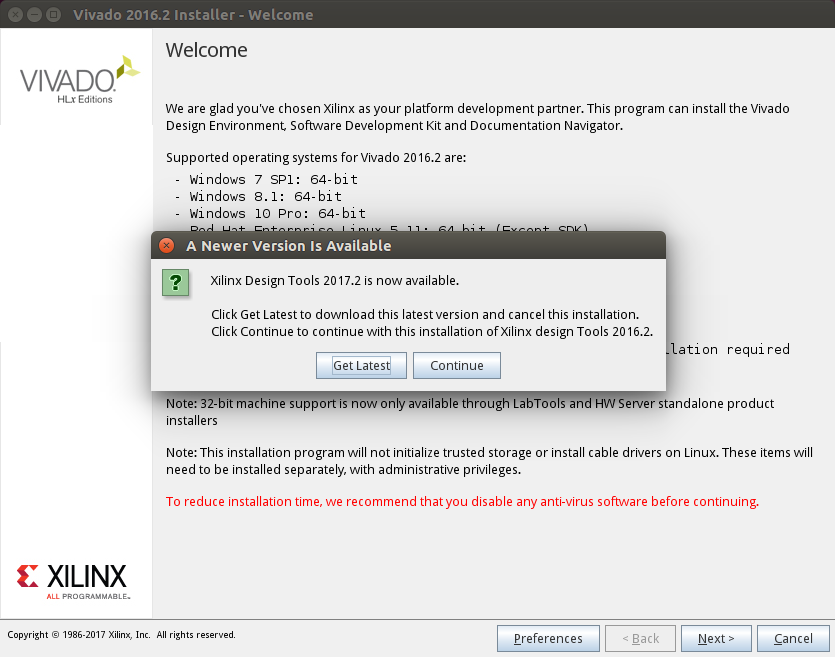
\includegraphics[width=1\textwidth,trim={0 8cm 0 8cm},clip]{images/devguide/vivado-install--1.png}
    \caption[Vivado: Step 1]{%
        Vivado: Step 1: It is very important to select "Continue"!
    }
    \label{fig:devguide:vivado1}
\end{figure}

\begin{figure}
    \centering
    \includegraphics[width=1\textwidth]{images/devguide/vivado-install-00.png}
    \caption[Vivado: Step 2]{%
        Vivado: Step 2
    }
    \label{fig:devguide:vivado2}
\end{figure}

\begin{figure}
    \centering
    \includegraphics[width=1\textwidth]{images/devguide/vivado-install-01.png}
    \caption[Vivado: Step 3]{%
        Vivado: Step 3
    }
    \label{fig:devguide:vivado3}
\end{figure}

\begin{figure}
    \centering
    \includegraphics[width=1\textwidth,trim={0 5cm 0 0cm},clip]{images/devguide/vivado-install-02.png}
    \caption[Vivado: Step 4]{%
        Vivado: Step 4
    }
    \label{fig:devguide:vivado4}
\end{figure}

\begin{figure}
    \centering
    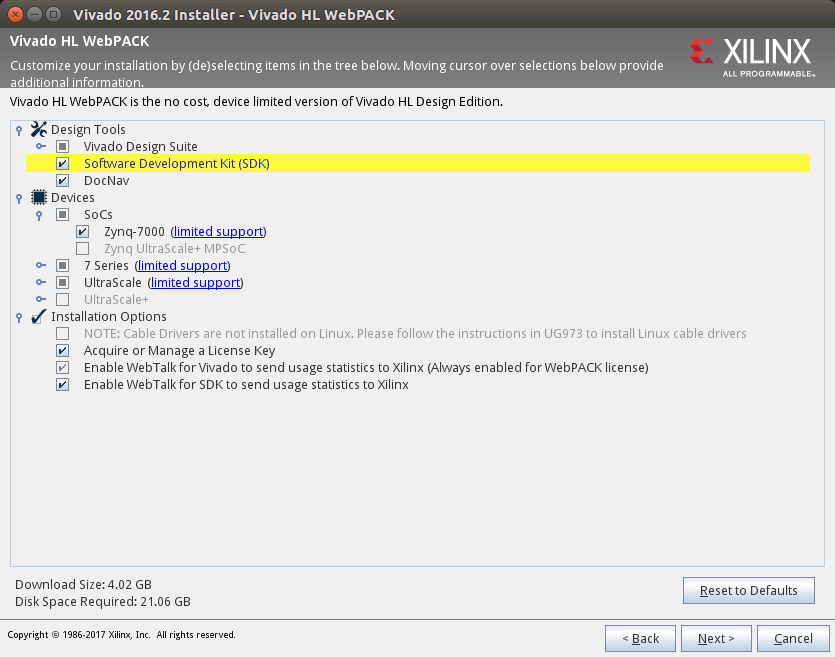
\includegraphics[width=1\textwidth,trim={0 6cm 0 0cm},clip]{images/devguide/vivado-install-04.png}
    \caption[Vivado: Step 5]{%
        Vivado: Step 5
    }
    \label{fig:devguide:vivado5}
\end{figure}

\begin{figure}
    \centering
    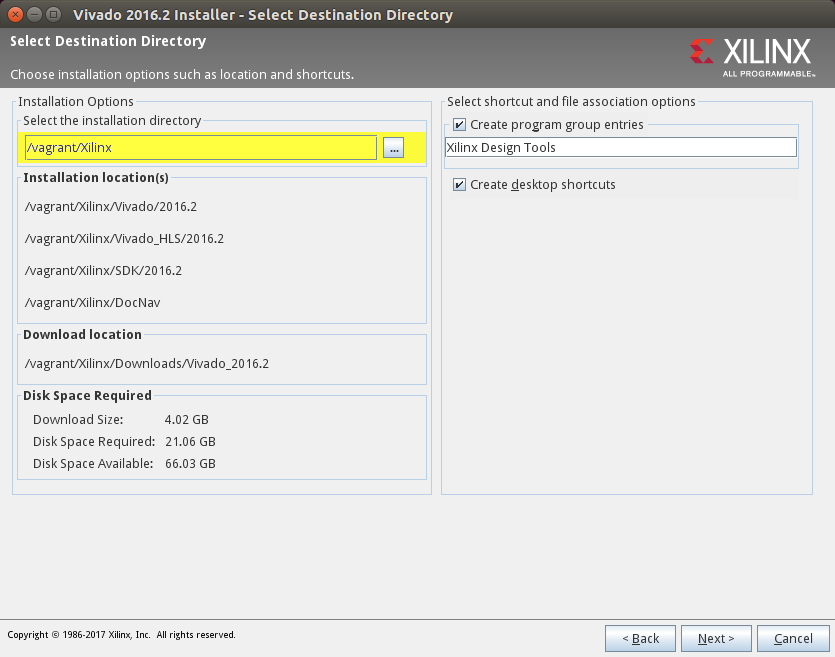
\includegraphics[width=1\textwidth]{images/devguide/vivado-install-05.png}
    \caption[Vivado: Step 6]{%
        Vivado: Step 6: Set the installation directory to \textit{/vagrant/Xilinx}
    }
    \label{fig:devguide:vivado6}
\end{figure}

\begin{figure}
    \centering
    \includegraphics[width=1\textwidth,trim={0 8cm 0 3cm},clip]{images/devguide/vivado-install-10.png}
    \caption[Vivado: Step 7]{%
        Vivado: Step 7
    }
    \label{fig:devguide:vivado7}
\end{figure}

\begin{figure}
    \centering
    \includegraphics[width=1\textwidth,trim={0 10cm 0 0cm},clip]{images/devguide/vivado-install-11.png}
    \caption[Vivado: Step 8]{%
        Vivado: Step 8
    }
    \label{fig:devguide:vivado8}
\end{figure}

\begin{figure}
    \centering
    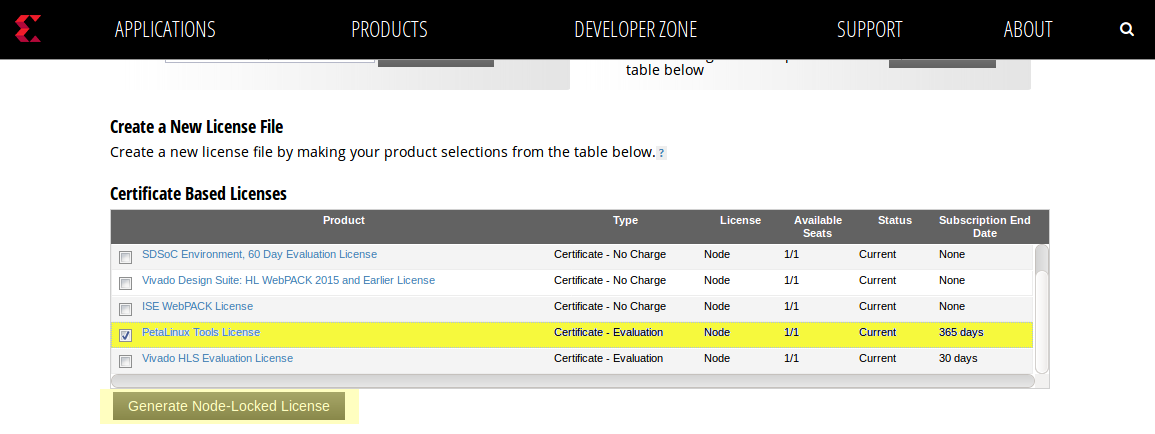
\includegraphics[width=1\textwidth]{images/devguide/vivado-install-12.png}
    \caption[Vivado: Step 9]{%
        Vivado: Step 9
    }
    \label{fig:devguide:vivado9}
\end{figure}

\begin{figure}
    \centering
    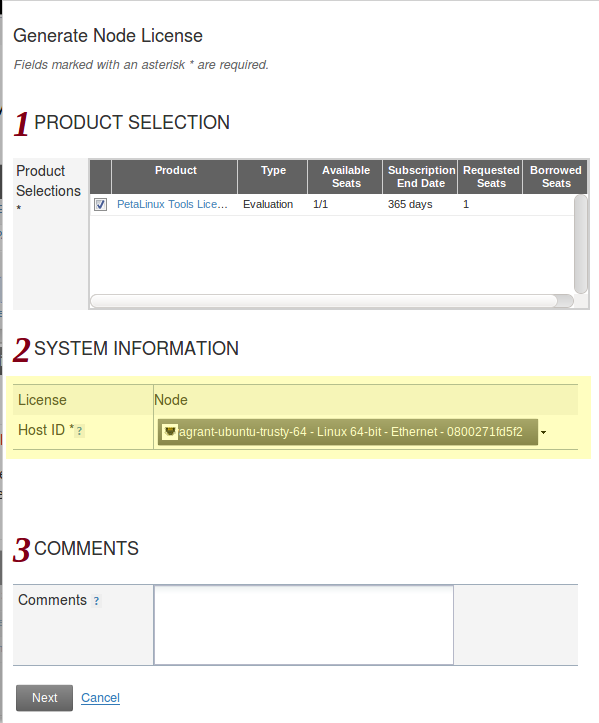
\includegraphics[width=1\textwidth,trim={0 8cm 0 8cm},clip]{images/devguide/vivado-install-14.png}
    \caption[Vivado: Step 10]{%
        Vivado: Step 10
    }
    \label{fig:devguide:vivado10}
\end{figure}

\begin{figure}
    \centering
    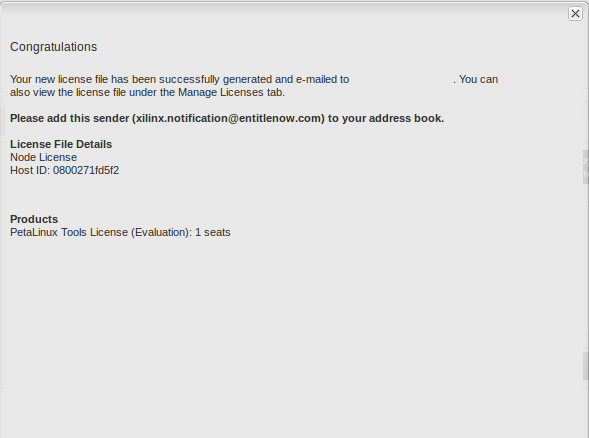
\includegraphics[width=1\textwidth,trim={0 8cm 0 0cm},clip]{images/devguide/vivado-install-16.png}
    \caption[Vivado: Step 11]{%
        Vivado: Step 11
    }
    \label{fig:devguide:vivado11}
\end{figure}

\begin{figure}
    \centering
    \includegraphics[width=1\textwidth]{images/devguide/vivado-install-17.png}
    \caption[Vivado: Step 12]{%
        Vivado: Step 12
    }
    \label{fig:devguide:vivado}
\end{figure}

\begin{figure}
    \centering
    \includegraphics[width=1\textwidth]{images/devguide/vivado-install-18.png}
    \caption[Vivado: Step 13]{%
        Vivado: Step 13
    }
    \label{fig:devguide:vivado}
\end{figure}

\begin{figure}
    \centering
    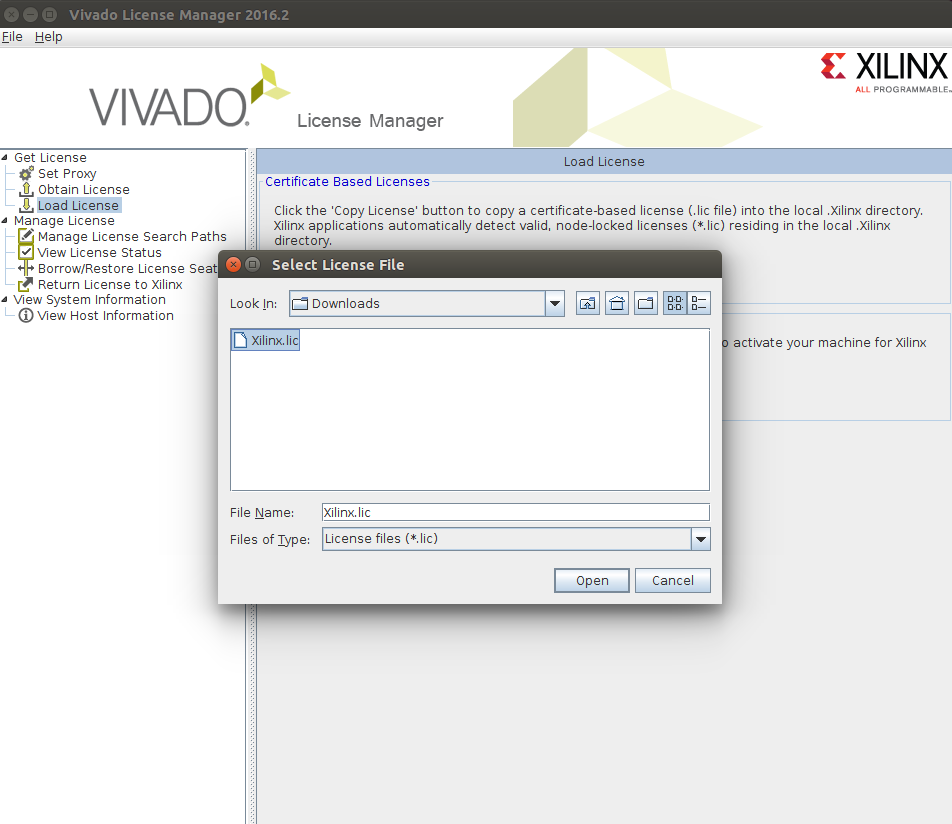
\includegraphics[width=1\textwidth,trim={0 8cm 0 8cm},clip]{images/devguide/vivado-install-19.png}
    \caption[Vivado: Step 14]{%
    Vivado: Step 14
    }
    \label{fig:devguide:vivado}
\end{figure}

\begin{figure}
    \centering
    \includegraphics[width=1\textwidth,trim={0 8cm 0 8cm},clip]{images/devguide/vivado-install-20.png}
    \caption[Vivado: Step 15]{%
    Vivado: Step 15
    }
    \label{fig:devguide:vivado}
\end{figure}

\begin{figure}
    \centering
    \includegraphics[width=1\textwidth,trim={0 8cm 0 8cm},clip]{images/devguide/vivado-install-22.png}
    \caption[Vivado: Step 16]{%
        Vivado: Step 16
    }
    \label{fig:devguide:vivado}
\end{figure}

\section{Building a Linux}
\label{sec:devguide:fpga_toolchain:linux}

With the fully set up build box it is possible to build an image with only two commands.
If new features are being added to the FPGA project or the server application is altered, of course the build steps can be performed, but an initial build is advisable.

First we copy the repo to a \textbf{non-shared} folder because uboot requires \textit{mmap()} which of course cannot handle shared folders.
And then we build the image in one go. This includes building the linux, the bitstream, the required firststage bootloader and the board support package, the logger kernel module, the server application, the scope application.
After that a bash script is used to create an image with all the components, mount it and provision the ubuntu environment.
Do do all of this do

\begin{listing}
    \begin{minted}[autogobble]{bash}
        cp -r /repo ~/local_folder
        cd ~/local_folder
        make init
    \end{minted}
\end{listing}

After the build has finished the image can be created using

\begin{listing}
    \begin{minted}[autogobble]{bash}
        cd ~/local_folder/firmware/arm
        sudo sh scripts/image.sh scripts/ubuntu.sh red-pitaya-ubuntu.img 1024
    \end{minted}
\end{listing}

Those scripts were initially created by the Red Pitaya corporation, altered by Pavel Demin\cite{TODO:} and altered by us to fit our needs.

TODO: references to vivado documentation
%>>>

\chapter{Filter Toolchain} % <<< --------------------------------------------- %
\label{ch:devguide:fpga_toolchain}
% ---------------------------------------------------------------------------- %
matlab stuff: What is where,  how do I specify a new filter,  how do I extract
the filters into Vivado, where can plot data be found
%>>>

\chapter{Server} % <<< ------------------------------------------------------- %
\label{ch:devguide:server}
% ---------------------------------------------------------------------------- %

The server application runs on the ARM Linux and is in charge of shoving data from the FPGA to the network and vice versa.
How it can be built and extended is explained in this section.

\section{Building the server}
\label{sec:devguide:server:build}

The server can only be built using the build environment explained in Chapter~\ref{ch:devguide:fpga_toolchain}.
A simple

\begin{listing}
    \begin{minted}[autogobble]{bash}
        cd /repo/firmware/arm/server
        make
    \end{minted}
\end{listing}

should suffice to build all the external dependencies and the binary for the ARM core.

The externals can be rebuilt using

\begin{listing}
    \begin{minted}[autogobble]{bash}
        cd /repo/firmware/arm/server
        make external
    \end{minted}
\end{listing}

and the server application can be rebuilt after changes using

\begin{listing}
    \begin{minted}[autogobble]{bash}
        cd /repo/firmware/arm/server
        make arm
    \end{minted}
\end{listing}

The server application is a one file application and depends on libuWebSockets\cite{TODO:} and a headerfile called json.hpp\cite{TODO:} which contains the entire JSON library.

There is two important functions for extending the server application: onHttpRequest and onMessage.

\subsection{onHttpRequest}

This callback gets called when the user makes an HTTP request wich is not an \textit{UPGRADE} request. Currently it simply serves the files from the filesystem, but could easily be extended to outline data or the likes.
Returning a correct HTTP Response has to be done manually and not well documented in the library itself.

If the response should outline a \textit{200 OK} status,

\begin{listing}
    \begin{minted}[autogobble]{C++}
        res->end(const char*, size_t);
    \end{minted}
\end{listing}

can be used with a string and a size. The lib then detects that no header is attached to the response and attaches a proper textit{200 OK} header.

If a custom header should be attached it first has to be attached and then the actual answer like so

\begin{listing}
    \begin{minted}[autogobble]{C++}
        std::string mime;
        char header[128];

        mime = std::string("text/css");
        std::string content = std::string("Hello World");
        int header_length = std::sprintf(
            header,
            "HTTP/1.1 200 OK\r\nContent-Length: %u\r\nContent-Type: %s\r\n\r\n",
            str.size(),
            mime.c_str()
        );
        res->write(header, header_length);
        res->end(str.c_str(), str.size());
    \end{minted}
\end{listing}

I am not entirely sure if better handling of this will follow in the future or if it is a performance thing, as the library itself is awesome in structure and tidyness. But docs sadly are very sparse

\subsection{onMessage}

This callback is triggered when a new message is received through the WebSocket.
For now in our project this call only handles incomming text messages as those conatin the instructions.
Binary messages are simply discarded but could be used at a later time to interface the DAC.

To add any new functionality, the code should be inspected and extended in analogy.

\section{Instruction Set}
\label{sec:devguide:server:instruction}

The instruction set contains TODO: commands which are listed in the lististings \ref{TODO:} downto \ref{TODO:}.

\subsection{Forcing a new trigger event}

This command forces the logger to finish it's current frame. It still repects the set pre and suf conditions.
The server does not automatically send the recorded frame. It has to be requested separately.
The argument needs to be always set to "true"

\begin{tcolorbox}[
    title={
        \refstepcounter{listing}
        Listing \thelisting: Forcing a new trigger event
        \label{lst:devguide:server:instr:1}
        \addcontentsline{lol}{listing}{\protect\numberline{\thelisting}Forcing a new trigger event}
    }
]
\inputminted[
    linenos,
    numbersep=4pt,
    style=solarizedlight,
]{javascript}{./code/serverinstructions/forceTrigger.js}
\end{tcolorbox}

\subsection{Configuring the frame the server sends}

This command tells the server how big the frame should be and how many samples have to be recorded before and after the trigger. All arguments have to be numbers in the JSON format, not strings.

\begin{tcolorbox}[
    title={
        \refstepcounter{listing}
        Listing \thelisting: Configuring the frame the server sends
        \label{lst:devguide:server:instr:2}
        \addcontentsline{lol}{listing}{\protect\numberline{\thelisting}Configuring the frame the server sends}
    }
]
\inputminted[
    linenos,
    numbersep=4pt,
    style=solarizedlight,
]{javascript}{./code/serverinstructions/frameconfig.js}
\end{tcolorbox}

\subsection{Setting the numbers of logged channels}

This command tells the server how many channels are being logged. This should always be two as the STEMlab does not support more channels. The logger itself would support up to 8 channels.
The argument has to be a number in the JSON format, not strings.

\begin{tcolorbox}[
    title={
        \refstepcounter{listing}
        Listing \thelisting: Setting the numbers of logged channels
        \label{lst:devguide:server:instr:3}
        \addcontentsline{lol}{listing}{\protect\numberline{\thelisting}Setting the numbers of logged channels}
    }
]
\inputminted[
    linenos,
    numbersep=4pt,
    style=solarizedlight,
]{javascript}{./code/serverinstructions/numberofchannels.js}
\end{tcolorbox}

\subsection{Reading the currently stored frame}

This command forces the server to send the currently stored frame over the binary channel as soon as the current frame is finished. If the logger is not recording currently the frame will be sent immediately.
The \textit{channel} argument has to be a number in the JSON format, not strings.

\begin{tcolorbox}[
    title={
        \refstepcounter{listing}
        Listing \thelisting: Reading the currently stored frame
        \label{lst:devguide:server:instr:4}
        \addcontentsline{lol}{listing}{\protect\numberline{\thelisting}Reading the currently stored frame}
    }
]
\inputminted[
    linenos,
    numbersep=4pt,
    style=solarizedlight,
]{javascript}{./code/serverinstructions/readframe.js}
\end{tcolorbox}

\subsection{Requesting a new frame and reading it when it is ready}
This command forces the server to start a new frame and send it over the binary channel as soon as the frame is finished.
The \textit{channel} argument has to be a number in the JSON format, not strings.

\begin{tcolorbox}[
    title={
        \refstepcounter{listing}
        Listing \thelisting: Requesting a new frame and read it when it is ready
        \label{lst:devguide:server:instr:5}
        \addcontentsline{lol}{listing}{\protect\numberline{\thelisting}Requesting a new frame and read it when it is ready}
    }
]
\inputminted[
    linenos,
    numbersep=4pt,
    style=solarizedlight,
]{javascript}{./code/serverinstructions/requestframe.js}
\end{tcolorbox}

\subsection{Setting the sampling rate}

This command sets the sampling rate.
The argument has to be a number in the JSON format and has to be the samplingrate in \si{\Hz}

\begin{tcolorbox}[
    title={
        \refstepcounter{listing}
        Listing \thelisting: Setting the sampling rate
        \label{lst:devguide:server:instr:6}
        \addcontentsline{lol}{listing}{\protect\numberline{\thelisting}Setting the sampling rate}
    }
]
\inputminted[
    linenos,
    numbersep=4pt,
    style=solarizedlight,
]{javascript}{./code/serverinstructions/samplingrate.js}
\end{tcolorbox}

\subsection{Polling the status of the logger}

This command requests the current logger status.
The response contains all the information the logger currently holds.

\begin{tcolorbox}[
    title={
        \refstepcounter{listing}
        Listing \thelisting: Polling the status of the logger
        \label{lst:devguide:server:instr:7}
        \addcontentsline{lol}{listing}{\protect\numberline{\thelisting}Polling the status of the logger}
    }
]
\inputminted[
    linenos,
    numbersep=4pt,
    style=solarizedlight,
]{javascript}{./code/serverinstructions/status.js}
\end{tcolorbox}

\subsection{Configuring the trigger}

This command configures the currently active trigger.
For now, only rising edge triggers are supported on the server side. The logger would support way more trigger types (For more information read the logger code).
Channel is the channel that should be triggered on.
Level is the level on which the trigger should shoot and slope is the minimal slope the curve needs to have.
Hysteresis is configured for all triggers at once and makes sure there is no accidential trigger. It is the variance the signal can have until a trigger gets armed.

\begin{tcolorbox}[
    title={
        \refstepcounter{listing}
        Listing \thelisting: Configuring the trigger
        \label{lst:devguide:server:instr:8}
        \addcontentsline{lol}{listing}{\protect\numberline{\thelisting}Configuring the trigger}
    }
]
\inputminted[
    linenos,
    numbersep=4pt,
    style=solarizedlight,
]{javascript}{./code/serverinstructions/trigger.js}
\end{tcolorbox}

%>>>

\chapter{Scope} % <<< -------------------------------------------------------- %
\label{ch:devguide:scope}
% ---------------------------------------------------------------------------- %
what is where, yarn, \ldots
%>>>

%^^A vim: foldenable foldcolumn=4 foldmethod=marker foldmarker=<<<,>>>
